\documentclass[letterpaper,fleqn,11pt]{report}
\usepackage[margin=0.75in]{geometry}
% Wait to usepackage these until they are needed.
% \usepackage{moreverb}
% \usepackage{float}
\usepackage{subfigure}
\usepackage{graphicx}
\usepackage{amsfonts, psfrag, fancyhdr, layout, appendix, subfigure, array}
\usepackage{wrapfig}
\usepackage{color}
\definecolor{gray}{gray}{0.25}
\usepackage[numbers]{natbib}
%\usepackage[nolist,nohyperlinks]{acronym}
\usepackage{url}
\usepackage{longtable}
\usepackage{fancyvrb}
\usepackage{moreverb} % for file listing

\usepackage[T1]{fontenc}
\usepackage[latin9]{inputenc}

\usepackage[pdftex,colorlinks=true,urlcolor=blue,citecolor=gray,linkcolor=gray]{hyperref}

% Set equal margins on book style
%\setlength{\oddsidemargin}{53pt}
%\setlength{\evensidemargin}{53pt}
%\setlength{\marginparwidth}{57pt}
%\setlength{\footskip}{30pt}

% Settings for the fancyhdr package
%
% Redefine plain page style
% \fancypagestyle{plain}{
% \fancyhf{}
% \renewcommand{\headrulewidth}{0pt}
% \fancyfoot[LE,RO]{\thepage}
% }

% Code for creating empty pages
% No headers on empty pages before new chaptermark
\makeatletter

% \def\cleardoublepage{\clearpage\if@twoside \ifodd\c@page\else
%     \hbox{}
%     \thispagestyle{plain}
%     \newpage
%     \if@twocolumn\hbox{}\newpage\fi\fi\fi}
% \makeatother \clearpage{\pagestyle{plain}\cleardoublepage}

% With the book style a new chapter always starts on an odd page. If
% the previous page is empty, the above code ensures that it is of
%\pagestyle{plain}.
%\pagestyle{fancy}
%\fancyhf{}
%\renewcommand{\chaptermark}[1]{\markboth{ \emph{#1}}{}}
% \fancyhead[]{}
% \fancyhead[RE]{}
%\fancyfoot[LE,RO]{\thepage}

% Dutch style of paragraph formatting, i.e. no indents.
\setlength{\parskip}{1.3ex plus 0.2ex minus 0.2ex}
\setlength{\parindent}{0pt}

% Again, uncomment when/if needed.
% % Define the \sourcelst command to create a floating listing of 
% % a (separate) source file.
% \newfloat{listing}{t}{lop}
% \floatname{listing}{Listing}
% \def\sourcelst#1#2{
% \begin{listing}
% \begin{tabular}{|@{\hspace{0.04\linewidth}}c@{\hspace{0.02\linewidth}}|}
% \hline \\
% \begin{minipage}{0.94\linewidth}
% \small\listinginput{1}{#1}
% \end{minipage}
% \\ \\ \hline
% \end{tabular}
% \caption{[{\tt #1}]\ \ #2}
% \label{lst:#1}
% \end{listing}
% }

\title{{\Huge Ames Albedo Reconstruction Software}\\
{\em Part of the NASA NeoGeography Toolkit}\\
Version 0.1}

\author{
Ara Nefian\\
Oleg Alexandrov\\
Zachary Moratto\\
\\
Intelligent Robotics Group\\
NASA Ames Research Center\\
}

\setcounter{chapter}{1} 
\renewcommand{\thesection}{\arabic{section}}
\renewcommand{\thefigure}{\arabic{figure}}
\renewcommand{\theequation}{\arabic{equation}}

\begin{document}

%\frontmatter
\maketitle
%\include{acknowledgments}
\tableofcontents

%\mainmatter

% Adjustments headers
%\fancyhead[LO]{\leftmark}
%\fancyhead[RE]{\emph{Chapter \thechapter}}

\newpage

\section{Overview}\label{overview}

The albedo reconstruction software takes the following inputs:
\begin{enumerate}
\item A set of DRG (Digital Raster Graphic) images of the Moon in the GeoTIFF format
\item A set of DEM (Digital Elevation Model) images in the GeoTIFF format
\item The Sun and spacecraft position at the moment each DRG image was
  taken. 
\end{enumerate}

The algorithm uses the Sun/spacecraft position and DEM data to
correct for the illumination conditions in the DRG images, thus
computing Moon's true albedo. 

In addition to creating albedo images, the software can also be used
for generating image mosaics (see the parameter REFLECTANCE\_TYPE in
section \ref{settings}). In that case, the DEM images and Sun/spacecraft positions are
not required.

\section{Compiling and running the albedo software}

The albedo reconstruction software needs to fetched from GitHub, using
the command:

\begin{verbatim}
  git clone https://github.com/NeoGeographyToolkit/PhotometryTK.git
\end{verbatim}
 
This will create a directory named \texttt{PhotometryTK}. The
\texttt{INSTALL} file in that directory has instructions for how to
compile and install the software and its pre-requisites.

The albedo reconstruction software can be called by using the script
{\it reconstruct.sh} in the directory PhotometryTK/src/tools.

The script is called as follows:

reconstruct.sh settings.txt labelStr

Here, {\it settings.txt} is the settings file (section \ref{settings}), and
{\it labelStr} is a string label. The output of running this command will be
stored in the directory {\it albedo\_labelStr}. This directory will have several subdirectories, with the following names and data:

\begin{itemize}
\item {\it albedo} --  a set of albedo tiles in the GeoTIFF format with pixel values between 0 and 255; the size of the tiles is specified in the settings file (section \ref{settings})
\item {\it albedo\_sub4} -- the albedo tiles at 1/4th the original resolution, together with a kml tree at this resolution that can be visualized in Google Earth\footnote{This directory is not generated when the software is run on multiple machines (section \ref{supercomp}) as kml generation is hard to parallelise and is best done offline.}
\item {\it error} --  the error map for each albedo tile (if
  COMPUTE\_ERRORS is set to 1, see section \ref{settings})
\item {\it DEM} --  the averaged DEM values for each albedo tile
\item {\it exposure} --  the estimated exposure time for each input DRG
  image (section \ref{algorithm})
\item {\it weight} --  the weights for each image
\end{itemize}

\section{Sample runs}\label{samples}

Two {\it sample runs} (settings files and other necessary input data)
are available in the directory PhotometryTK/src/photk/tests. They are executed automatically if the user
runs {\it make check} in PhotometryTK/build.


\section{Running the software on multiple machines}\label{supercomp}

The albedo reconstruction software can be distributed over a very large number of computing
nodes (using GNU parallel), as long as those nodes use the same filesystem. The
computing nodes need to be specified in a file, with one machine name
per line, and the environmental variable PBS\_NODEFILE should be set to
the path to this file. \footnote{On NASA's Pleiades Supercomputer the
variable PBS\_NODEFILE is set automatically.} If this variable is not defined, the jobs are
only run on the current machine. 
 
The parameter NUM\_PROCESSES in the settings file (section \ref{settings}) can be used
to control how many processes to start on a given computing node. This number depends
on the number of cores available on the node, the amount of memory available, and the resolution of the input images
(higher resolution requires more memory and therefore fewer processes can be run simultaneously on a node).

\section{The settings file}\label{settings}

The parameters controlling the albedo reconstruction software are specified in a
settings file (a sample settings file is shown in the appendix). It has the following entries:

\begin{longtable}{ l p{7cm} }
DRG\_DIR & The path to the directory of DRG images. \\
\\
DEM\_DIR & The path to the directory of DEM images. \\
\\
SUN\_POSITION\_FILE  & The Sun position file.  \\
\\
SPACECRAFT\_POSITION\_FILE & The spacecraft position file.  \\
\\
NUM\_PROCESSES & How many simultaneous processes to start on a given
computing node. \\
\\
TILE\_SIZE & Output albedo tile size, in degrees (usually 4 by 4 degrees). \\
\\
SIMULATION\_BOX &         The region in which to compute the albedo, in
the format lon\_min : lon\_max : lat\_min : lat\_max. If this
parameter is not provided, the region will be assumed to be the entire Moon. \\
\\
REFLECTANCE\_TYPE &
The reflectance type. Values: 0 -- the reflectance is not
be used, the result of albedo reconstruction is just an image mosaic, 1 --
the Lambertian reflectance model is used, 2 -- the Lunar-Lambertian
reflectance model (Equation~\ref{reflectance}) is used.\\
\\
SHADOW\_THRESH    &         
 Shadow threshold, with values between 0 to 255 (the input DRG images
 have values between 0 to 255, see section \ref{requirements}). Its
 use depends on the parameter SHADOW\_TYPE.
\\
\\
SHADOW\_TYPE & Determines how to classify which input DRG image pixels are in
the shadow (section \ref{algorithm}). Values: 0 -- no pixels are in
the shadow, 1 -- pixels in the shadow are those with values below
SHADOW\_THRESH, this is the default. Advanced values: 2 -- pixels in the
shadow satisfy $I/(R\cdot T) < t$ \footnote{$I$ is the
image value, $R$ is the Lambertian reflectance, $T$ is the image
exposure, and $t$ is the shadow threshold.}, 3 -- 
analogous to option 2, but use the Lunar-Lambertian reflectance model (Equation~\ref{reflectance})
instead of the Lambertian model.\\
\\
TR\_CONST & A constant which determines how bright the albedo will be, a larger value will make the albedo 
appear darker. \\
\\
PHASE\_COEFF\_C1  & The coefficient $c_1$ in reflectance formula (Equation~\ref{reflectance}).\\
\\
PHASE\_COEFF\_C2  & The coefficient $c_2$ in the same expression.\\
\\
MAX\_NUM\_ITER     &
Maximum number of albedo update iterations. If it is equal to 0, the image
exposure, phase coefficients, and the albedo itself will only be
initialized, and no subsequent iterations will take place to improve
the initial values (see the algorithm in section \ref{algorithm}).\\ 
\\
NO\_DEM\_DATA\_VAL &
The value used in the DEM images to denote that no data is available at the
current pixel. This number is normally stored within the DEM images;
only if it absent there will the value specified here be used.\\
\\
USE\_WEIGHTS &
 If to use weights to seamlessly blend the albedo values obtained from
 individual images (1 means true, and 0 means false). See section \ref{algorithm}.\\
\\
USE\_NORMALIZED\_COST\_FUN &
 If to enforce that the sum of weights over all images add up to 1 at
 each pixel.  If true, all pixels will contribute in equal amount to
 the cost function (Equation~\ref{cost_function}). This flag makes a difference only if multiple
 albedo iterations are performed (MAX\_NUM\_ITER $>$ 0). Turning this
 on incurs a significant performance hit.\\
\\
COMPUTE\_ERRORS   &
 If at the end of the algorithm to compute the albedo error map (Equation~\ref{albedo_error}), showing at each pixel what the error was in computing the albedo at that pixel.\\
\\
% UPDATE\_HEIGHT   &
%  If to update the terrain height based on the computed albedo (this is an experimental feature, not yet fully supported).\\
% \\

\end{longtable}

\section{Requirements for the input}\label{requirements}

As mentioned in section \ref{overview}, the inputs to the albedo reconstruction software are a set of DRG images, a set of DEM images, and the Sun and spacecraft position for each DRG image. Here we specify the exact requirements for the data as expected by the software.

\begin{enumerate}

\item The DRG images should be in a directory and stored in the GeoTIFF format. It is assumed that the intensity values for each image pixel are between 0 and 255 (uint8).  The first 11 characters of each image in that directory should be unique, and will be the means by which we will later look up the Sun and spacecraft position for that image. For example, given the image:

DRG\_input\_sub64/AS15-M-0074\_0075-DRG.tif

the lookup key is the 11-character string: AS15-M-0074.

\item The DEM images should be in a directory and stored in the GeoTIFF
format. They may or may not overlap. If the DEM images overlap, the
values from all images at a given pixel will be averaged. It is expected
that the DEM images are either in int16 or float format. If the
images lack the No Data Value, it should be explicitly set in the
settings file using the parameter NO\_DEM\_DATA\_VAL (section \ref{settings}).

\item The Sun positions for the DRG images should be listed in a text file,
 with one line in the file for each DRG image. The same should
hold for the spacecraft position. Each line in these lists needs to
be in the format: 

lookup\_key x y z

where lookup\_key is the 11-character string that identifies the DRG
image, and x, y, and z are the coordinates of the Sun (spacecraft)
 in the Cartesian coordinate system whose origin is the center of the
 Moon. The values should be in kilometers. An example entry for the Sun
 position is 

AS15-M-0074 -1345328.6130903 151849061.51791 689530.60102555

\item The directories containing the DRG and DEM images should be
  user-writeable, as the software will create in those directories a
  list of the GeoTIFF images contained within them, together with the
  coordinates of the corners of each image. These lists are created
  only once and speed up subsequent computations.

\end{enumerate}

Sample runs with the inputs satisfying these requirements are available (section \ref{samples}).

\section{Modeling and the algorithm}\label{algorithm}

In section we describe the mathematical modeling underlying the albedo reconstruction software.

Let $I^k_{ij}, A_{ij}$, $R^k_{ij}, T^k$ be the
observed image value, albedo, reflectance, and exposure time. Here, $(i,j)$ are pixel indices, and $k$ is the
image index.

We would like to determine the set ${\tilde{A}_{ij}, \tilde{T}^k},
\tilde{c}_l = \arg \min_{A_{ij}, T^k, c_l} {\bf Q}$  where
\begin{eqnarray}
{\bf Q} = \sum_k\sum_{ij}\left[(I^k_{ij}-A_{ij}T^kR^k_{ij})^2 S^k_{ij}w^k_{ij}\right]
\label{cost_function}
\end {eqnarray}
Here,  $S^k_{ij}$ is a shadow binary variable, $S^k_{ij} =
0$ when the pixel $(i, j)$ is in the shadow and 1 otherwise. The weights
$w^k_{ij}$ are chosen such that they have linearly decreasing values
from the center of the image ($w^k_{ij} = 1$) to the image boundaries
($w^k_{ij} = 0$). The choice of these weighs insures that the
reconstructed albedo mosaic is seamless. 

\begin{figure}[ht]
\centerline{\frame{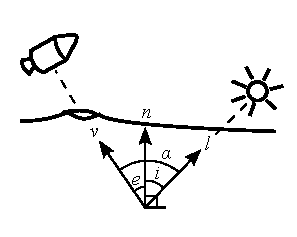
\includegraphics[width=5.5cm]{images/angles.pdf}}}
\caption{Illumination and viewing angles used by the Lunar-Lambertian reflectance model.}
\label{fig:angles}
\end{figure}

In the above equation the reflectance is computed using the Lunar-Lambertian model and is given by
\begin{eqnarray}
R^k_{ij} = (e^{-c_1\alpha} + c_2)\left[ (1-L(\alpha))\cos({\bf i}_{ij}^k)
  +2L(\alpha)\frac{\cos({\bf i}_{ij}^k)}{\cos({\bf i}_{ij}^k) +
    \cos({\bf e}_{ij}^k)} \right]
\label{reflectance}
\end {eqnarray}
where $L(\alpha) = 1 + A\alpha + B\alpha^2 + C\alpha^3$ is a weighting factor between the Lunar and Lambertian reflectance models that depends on the phase angle ($\alpha$), ${\bf i}_{ij}^k$ and ${\bf e}_{ij}^k$
are the incident and emission angles at image $k$ and pixel
$(i,j)$ (see Figure~\ref{fig:angles}). The numbers $c_1$ and $c_2$ are called the {\it phase coefficients}.

Determining the best albedo reconstruction from a set of images and
the corresponding DEM (digital elevation map) is formulated as a cost function minimization
problem for the albedo $A_{ij}$, image exposures $T_k$, and phase
coefficients $c_1$ and $c_2.$ (Equation~\ref{cost_function}). An iterative solution to the above least square problem is given by the Gauss-Newton updates described below. 

\begin{itemize}
\item {\bf Step 1 (initialization)}: Compute the average DEM and the weights.
Normalize the weights so that the sum of weights at each pixel is 1 if the
parameter USE\_NORMALIZED\_COST\_FUN is set to 1 in the settings file
(section \ref{settings}). 
  Initialize the exposure time as inversely proportional to the average image
  reflectance. Initialize the phase coefficients $c_1$ and $c_2$ to some
  reasonable values. Initialize the albedo as the $\arg \min$ of the
  cost function {\bf Q} for fixed exposure time and phase
  coefficients 
\begin{eqnarray}
A_{ij} = \frac{\sum_k I_{ij}^k T^kR^k_{ij} S^k_{ij}w^k_{ij}}{\sum_k (T^k R^k_{ij})^2 S^k_{ij}w^k_{ij}}
\label{albedo_init}
\end{eqnarray}

\item {\bf Step 2}: Re-estimate the exposure time using
\begin{eqnarray}
\tilde{T} ^k = T^k + \frac{\sum_{ij} (I_{ij}^k-A_{ij}T^kR^k_{ij})A_{ij}R^k_{ij}S^k_{ij}w^k_{ij}}{\sum_{ij}(A_{ij} R^k_{ij})^2 S^k_{ij}w^k_{ij}}
\label{exposure_iter}
\end {eqnarray}

\item {\bf Step 3}: Re-estimate the phase coefficients using
\begin{eqnarray}
\tilde{c_1} = c_1 + \frac{\sum_{ijk}
  (I_{ij}^k-A_{ij}T^kR^k_{ij})A_{ij}T^k \frac{\partial R^k_{ij}}{\partial c_1}S^k_{ij}w^k_{ij}}{\sum_{ijk}\left(A_{ij}T^k\frac{\partial R^k_{ij}}{\partial c_1}\right)^2 S^k_{ij}w^k_{ij}}
\label{phasecoeff_iter}
\end {eqnarray}
and analogously for $c_2$. The partial derivatives $\partial
R^k_{ij}/\partial c_1$ and $\partial R^k_{ij}/\partial c_2$ are
computed from Equation~\ref{reflectance}.

\item {\bf Step 4}: Re-estimate the albedo using
\begin{eqnarray}
\tilde{A}_{ij}=A_{ij}+\frac{\sum_k (I_{ij}^k-A_{ij}T^kR^k_{ij}) T^kR^k_{ij}S^k_{ij}w^k_{ij}}{\sum_k (T^k R^k_{ij})^2 S^k_{ij}w^k_{ij}}
\label{albedo_iter}
\end {eqnarray}

\item {\bf Step 5}: Compute the error cost function $\bf Q$ for the re-estimated values of the albedo and exposure time.

\item {\bf Convergence}: If the convergence error between the consecutive iterations falls below a fixed threshold then stop. Otherwise return to step 2.

\item {\bf Step 6}: Estimate the accuracy of the albedo reconstruction
  at each pixel using the formula
\begin{eqnarray}
E_{ij}=\frac{\sum_k (I_{ij}^k/(T^k R^k_{ij})-A_{ij}) ^2S^k_{ij}w^k_{ij}}{\sum_k w^k_{ij}}
\label{albedo_error}
\end {eqnarray}

\end{itemize}

\section{Advanced usage}

The script {\it reconstruct.sh} computes the albedo by performing a
series of calls to the executable
{\it PhotometryTK/build/src/tools/reconstruct}. Advanced users may call this
program directly to execute a certain stage of the algorithm (section \ref{algorithm}).

The {\it reconstruct} executable takes the following options:

\begin{verbatim}
  -s [ --settings-file ] arg     Settings file
  -r [ --results-directory ] arg Results directory
  -f [ --images-list ] arg       The list of images
  -t [ --tiles-list ] arg        The list of albedo tiles
  -i [ --image-file ] arg        Current image or tile
  --initial-setup                Initial setup
  --save-weights                 Save the weights
  --compute-weights-sum          Compute the sum of weights at each pixel
  --init-dem                     Initialize the DEM
  --init-exposure                Initialize the exposure times
  --init-albedo                  Initialize the albedo
  --update-exposure              Update the exposure times
  --update-tile-phase-coeffs     Update the phase coefficients per tile
  --update-phase-coeffs          Update the phase coefficients by combining the
                                 results over all tiles
  --update-albedo                Update the albedo
  --compute-errors               Compute the errors in albedo
  --is-last-iter                 Is this the last iteration
  -h [ --help ]                  Display this help message
\end{verbatim}

For example, to initialize the exposure times for a given image, one may
issue the command:

reconstruct -s settings.txt -r albedo\_run -f albedo\_run/imagesList.txt -t albedo\_run/albedoTilesList.txt --init-exposure -i DRG\_DIR/AS16-M-2961.tif

Each time the {\it reconstruct} executable is run, it echoes the precise
command and options which were used to call it, so these calls can be
inferred by looking at the output of {\it reconstruct.sh}. 

\section{Retrieving the input data from ISIS cubes}

The albedo reconstruction software assumes that the input DRG images are in GeoTIFF
format, and that the sun and spacecraft positions are in text files (section \ref{overview}).
This section describes how to get this data from ISIS cubes.

The DRG images can be obtained by orthoprojecting the ISIS cubes 
onto the terrain data (a set of DEM tiles) using the script named {\it orthoproject\_cube.sh} in
the directory PhotometryTK/src/tools. The script assumes that the following packages
are installed: Ames Stereo Pipeline, ISIS libraries, and the GDAL
tools. The paths to them can be set in the script. It can be called
as:

orthoproject\_cube.sh input.cub input\_isis\_adjust DEM\_dir mpp num\_proc output.tif 

The arguments passed to it are, respectively, the cube file to
orthoproject, the ISIS adjust file storing the adjusted camera
position, the directory containing the DEM tiles to orthoproject onto, 
the desired output resolution in meters per pixel, the
number of processors to use, and the name of the output image.

To get the sun and spacecraft position from a list of ISIS cubes, the
script {\it get\_sun\_or\_spacecraft\_position.pl} is used, also located in PhotometryTK/src/tools.
The usage is: 

get\_sun\_or\_spacecraft\_position.pl sun-or-spacecraft inputCubesList.txt outputPositionList.txt

%\renewcommand{\thesection}{A}

\appendix

\renewcommand{\thesection}{A-\arabic{section}}


\section{A sample settings file}

\begin{verbatim}
# Files/directories
DRG_DIR                   DIM_input_2560mpp
DEM_DIR                   DEM_tiles_sub64
SUN_POSITION_FILE         meta/sunpos.txt 
SPACECRAFT_POSITION_FILE  meta/spacecraftpos.txt

# Constants
NUM_PROCESSES             8
TILE_SIZE                 4.0
SIMULATION_BOX            -180:180:-180:180
REFLECTANCE_TYPE          2
SHADOW_THRESH             40
SHADOW_TYPE               1
TR_CONST                  1.5
PHASE_COEFF_C1            1.7
PHASE_COEFF_C2            0.4
MAX_NUM_ITER              0
NO_DEM_DATA_VAL           -32767

# Actions
USE_WEIGHTS               1
USE_NORMALIZED_COST_FUN   0
COMPUTE_ERRORS            1
\end{verbatim}

% Create the References list
\bibliographystyle{plainnat}
\phantomsection % to make hyperref behave
%\addcontentsline{toc}{chapter}{\bibname}
\bibliography{bibliography}


\end{document}
